\documentclass[a4paper,10pt]{scrartcl}
\usepackage[backend=biber,bibencoding=utf-8]{biblatex}

\usepackage{praeambel}

%%% Eigene Daten: Beginn
\title{Portfolio}
\newcommand\authorA{Sebastian Schramm}
\newcommand\matrikelnrA{-}
\newcommand\modul{Informatik}
\newcommand\pruefer{-}
\date{\today}
%%% Eigene Daten: Ende

\begin{document}
\selectlanguage{ngerman}
\begin{titlepage}
  \pagestyle{empty}
  \centering

  \vspace*{0.5cm}
  \begin{otherlanguage*}{ngerman}
    \begin{sffamily} {
        \Large
        Hochschule -\\[1em]
        Fakultät IV -- Technische Informatik\\[0.1em]
        Modul: \modul\\[0.1em]
        Professor: \pruefer\\[0.1em]
      }
    \end{sffamily}
  \end{otherlanguage*}

  \vspace*{3cm}

  \begin{sffamily}
    \huge \bfseries
    \makeatletter
    \@title
    \makeatother
    \\
  \end{sffamily}

  \vspace*{1cm}

  \begin{otherlanguage*}{ngerman}
    
    \vspace*{3cm}
    
    von\\[0.75em]
    {
      \large
      \textbf{\authorA}\quad Matrikel-Nr. \matrikelnrA\\
      %\textbf{\authorB}\quad Matrikel-Nr. \matrikelnrB

      \vspace*{2cm}
      \makeatletter
      \@date
      \makeatother
    }
    \vfill
  \end{otherlanguage*}
\end{titlepage}

\tableofcontents

\newpage

%%% Protokoll: Beginn

\section{Deckblatt}
Deckblatt mit Ihrem vollständigen Namen, Matrikelnummer, Semester, Studiengang und Ihre unterschriebene Erklärung, dass Sie das Portfolio selbständig verfasst und nur die angegebenen Quellen und Hilfsmittel benutzt haben. Wörtlich oder dem Sinn nach aus anderen Werken entnommene Stellen sind unter Angabe der Quellen kenntlich zu machen.
\section{Was ist Informatik}
Schreiben Sie einen Aufsatz zum Thema „Was ist Informatik“. Dieser Aufsatz sollte maximal 1500 Zeichen lang sein (ca. eine DIN A4 Seite).\\
\\
Was ist Informatik	
Der Begriff Informatik setzt sich aus dem Wort Information und Automatik zusammen. „Die Kernaufgabe der Informatik befasst sich generell mit der Speicherung, Verarbeitung, Darstellung aber auch mit der Übertragung von Informationen.“ (Informatik Aufgaben. 2021) 
Zudem gibt es verschiedene Bereiche in der Informatik, wie die 
Theoretische Informatik, welche das Rückgrat bildet. Sie befasst sich mit den abstrakten und mathematikorientieren Aspekten der Informatik. Dazu zählen die Automatentheorie, Berechenbarkeitstheorie, Komplexitätstheorie und Quantencomputer. 
Bei der Praktischen Informatik geht es um die Entwicklung von Konzepten und Methoden zur Problemlösung in der realen Welt. Dabei ist eines der zentralen Themen die Softwaretechnik wo Konzepte für große Softwareprojekte entworfen werden. 
In der Technischen Informatik befasst man sich hauptsächlich mit den hardwareseitigen Grundlagen. (vgl, Informatik. 2021) Dazu zählen „[…] Mikroprozessortechnik, Rechnerarchitektur, eingebetteten und Echtzeitsystemen, Rechnernetzen.“ (Informatik. 2021) 
Auch ein sehr wichtiges Teilgebiet ist die Angewandte Informatik. Denn sie Beschäftigt sich mit der Anwendung in Informatikfremden Gebieten, wie die Biologie, Betriebswirtschaft und Medizin. Entsprechende Bereiche könnten die Computergrafik, Simulation und Datenverarbeitung sein.
(vlg, Angewandte Informatik. 2021) Zudem haben Informatiksysteme eine starke Auswirkung auf unsere heutige Gesellschafft. 

\begin{lstlisting}
	https://www.alphajump.de/karriereguide/beruf/aufgaben-informatik
	https://de.wikipedia.org/wiki/Informatik
	https://de.wikipedia.org/wiki/Angewandte_Informatik

	https://www.uni-halle.de/informatik/
\end{lstlisting}
\section{Persönlichkeit der Informatik}
Schreiben Sie einen Aufsatz über eine Persönlichkeit der Informatik. Dieser Aufsatz sollte maximal 1500 Zeichen lang sein (ca. eine DIN A4 Seite).\\
\\
Konrad Zuse und seine Errungenschaften
Konrad Ernst Otto Zuse war ein deutscher Bauingenieur, Erfinder und Unternehmer der Zuse KG. Konrad Zuse wurde am 22. Juni 1910 in Deutsch-Wilmersdorf geboren und starb am 18. Dezember 1995 in Hünfeld. Zuse baute 1941 „den ersten funktionstüchtigen, vollautomatischen, programmgesteuerten und frei programmierbaren, in binärer Gleitkommarechnung arbeitenden Rechner und somit den ersten funktionsfähigen Computer der Welt“(Wiki, 2021).
Aufgrund der monotonen und mühseligen Berechnungen im Bauingenieurwesen, wollte Zuse diese Arbeit automatisieren. Er entschloss sich 1935, seinen Beruf als Statiker zu kündigen und widmete sich der Entwicklung eines mechanischen Gehirns. 1937 wurde der erste mechanische Rechner Z1 fertiggestellt und basierte auf dem Binärsystem. Zusätzlich besaß der Z1„ein Ein-/Ausgabewerk, ein Rechenwerk, ein Speicherwerk und ein Programmwerk, das die Programme von gelochten Kinofilmstreifen ablas“(Wiki, 2021). Zuse entwickelte Methoden auf der Grundlage von Mantisse und Exponenten, dies Ermöglichte dem Z1 mit Gleitkommazahlen zu arbeiten (vgl. Wiki, 2021). Aufgrund der Unzuverlässigkeit des Z1, musste Zuse eine Alternative für die Schaltelemente finden.  Dadurch entstand der Z2 welcher nun Relais verwendet. 1941 wurde der Z3 vollendet welcher der erste elektrisch Programmiergare Computer der Welt war, welcher aber 1943 bei einem Bombenangriff zerstört wurde (vgl. Mark und Eniac, 2900).

\begin{lstlisting}
	https://de.wikipedia.org/w/index.php?title=Konrad_Zuse&oldid=204389120
	https://homecomputermuseum.de/historie/konrad-zuses-z1-z4/
\end{lstlisting}
\section[Dezimalzahlen in Hexadezimalsystem]{Wandeln Sie die folgenden Dezimalzahlen in das Hexadezimalsystem um: 2989, 57005, 48879.}
\begin{itemize}
	\item 2989	:	16	=	186	|Rest	2989	-16	*	486	=	13
	\item 186	:	16	=	11	|Rest	186		-16	*	11	=	10
	\item 11	:	16	=	0	|Rest	11
\end{itemize}
2989	= 	BAD\
\begin{itemize}
	\item 57005	:	16	=	3562|Rest	57005	-16	*	3562=	13
	\item 3562	:	16	=	222	|Rest	3562	-16	*	222	=	10
	\item 222	:	16	=	13	|Rest	222		-16	*	13	=	14
	\item 13	:	16	=	0	|Rest	13
\end{itemize}
57005	=	DEAD\
\begin{itemize}
	\item 48879	:	16	=	3054|Rest	48879	-16	*	3054=	15
	\item 3054	:	16	=	190	|Rest	3054	-16	*	190	=	14
	\item 190	:	16	=	11	|Rest	190		-16	*	11	=	14
	\item 11	:	16	=	0	|Rest	11
\end{itemize}
48879	=	BEEF\
\section[Äquivalenz mit XOR]{Wie zeigen Sie, die Äquivalenz der folgenden Ausdrücke mit XOR}
(x\vee y)\wedge \neg(x\wedge y)\\
\begin{tabular}[h]{c|c|c|c|c}
	x & y & (x\vee y) & \neg(x\wedge y) & a\wedge b \\
	\hline
	0 & 0 & 0 & 1 & 0 \\
	0 & 1 & 1 & 1 & 1 \\
	1 & 0 & 1 & 1 & 1 \\
	1 & 1 & 1 & 0 & 0 \\
\end{tabular}\\
\neg((x\wedge y)\vee(\neg x\wedge \neg y))\\
\begin{tabular}[h]{c|c|c|c|c}
	x & y & (x\wedge y) & (\neg x\wedge \neg y) & \neg(a\vee b) \\
	\hline
	0 & 0 & 0 & 1 & 0 \\
	0 & 1 & 0 & 0 & 1 \\
	1 & 0 & 0 & 0 & 1 \\
	1 & 1 & 1 & 0 & 0 \\
\end{tabular}\\
\neg(x\wedge y)\wedge(x\vee y)\\
\begin{tabular}[h]{c|c|c|c|c}
	x & y & \neg(x\wedge y) & (x\vee y) & a\wedge b \\
	\hline
	0 & 0 & 0 & 1 & 0 \\
	0 & 1 & 1 & 1 & 1 \\
	1 & 0 & 1 & 1 & 1 \\
	1 & 1 & 1 & 0 & 0 \\
\end{tabular}
\section{UML}
Schreiben Sie einen Aufsatz zum Thema „UML“. Dieser Aufsatz sollte maximal 3000 Zeichen lang sein (ca. zwei DIN A4 Seiten).\\
\\
UML
Während der Blüte der Objekt orientierten Programmierung in den 1990er Jahren, kamen vermehrt Vorschläge für eine Modellierungssprache. Die drei Grady Booch, Ivar Jacobson und James Rumbaugh hatte bereits ihre eigene Modellierungssprache entwickelt. Während sie zusammen bei Rational Software beschäftigt waren, kam ihnen kam die Idee, die verschiedenen Notationssysteme zusammenzuführen. Als Resultat entstand die UML. Die UML oder auch Unified Modeling Language ist eine Objektorientierte Sprache und besitzt Notationen zur Beschreibung von Softwaresystemen. Der Grundgedanke hierbei, ist eine einheitliche Notation für alle Softwaresysteme. (vgl. UML, 2021) Sie dient zur “Spezifikation, Konstruktion, Dokumentation und Visualisierung von Software-Teilen und anderen Systemen“ (UML, 2020). In der UML gibt es Notationselemente, aus denen sich verschiedene Diagramme erzeugen lassen. Im Jahre 1999 stieß OMG die Entwicklung von UML 2.0 an. Dabei verdeutlicht jedes Diagramm eine bestimmte Perspektive auf das zu modellierende System und kann dem Entwickler, oder Nutzer einen guten Überblick auf die Software verschaffen.
Es gibt verschiedene Modellierungssprachen, wie das Aktivitätsdiagramm welches die Ablaufmöglichkeiten eines Systems beziehungsweise Anwendungsfalls mit Aktionen darstellt. Wobei eine Aktion einen einzelnen Schritt darstellt und mit Kanten wird der Kontrollfluss angegeben.
Bei einem Anwendungsfalldiagramm oder auch Use Case Diagram, wird das Verhalten eines Systems aus der Benutzersicht dargestellt. Diese beschreiben aber auch die geplante Funktionalität eines Systems. Anschließend wird noch ein Akteur benötigt, dieser kann zum Beispiel eine Person oder ein System sein und gibt an, was dieses System tun soll. (vgl. UML, 2021)
Bei einem Klassendiagramm werden die Beziehungen zwischen den einzelnen Klassen verdeutlicht sowie, welche Attribute und Methoden in der jeweiligen Klasse vorhanden sind. Zusätzlich ist noch ersichtlich um welche Datentypen es sich handelt und welche Attribute/Methoden public, private oder protected sind. Mit der Generalisierung wird angegeben in welcher Beziehung die jeweiligen Klassen zueinander stehen, dies wird mit einer durchgezogenen Linie und einem Pfeil an einer der beiden enden dargestellt. Der Pfeil gibt an von welcher Klasse geerbt wird. (vgl. Klassendiagramm, 2021)
Ein Zustandsdiagramm beschreibt den Lebenszyklus der Objekte einer Klasse und ist eine graphische Darstellung eines Zustandsautomaten welche auf dem Konzept der endlichen Automaten basieren. Mithilfe eines Zustandsdiagrammes kann dargestellt werden, in welchem zustand sich das betrachtete Objekt befindet und welches Verhalten dieses Objekt in einer aktiven Klasse modelliert. (vgl. Endlicher Automat, 2021)

\begin{lstlisting}
	Unified Modeling Language. (19. Oktober 2020). In Wikipedia. Abgerufen am 4. Februar 2021, unter https://de.wikipedia.org/wiki/Unified_Modeling_Language
	Klassendiagramm. (9. Dezember 2020). In Wikipedia. Abgerufen am 4. Februar 2021, unter https://de.wikipedia.org/wiki/Klassendiagramm
	Endlicher Automat. (20. Januar 2021). In Wikipedia. Abgerufen am 4. Februar 2021, unter https://de.wikipedia.org/wiki/Endlicher_Automat
\end{lstlisting}
\section{zweiKonzentrischeQuadrate}
Damit dieses Programm funktioniert gehen dir davon aus, dass wir oben Links starten. Also bei 0,0 und unser Startrichtung nach rechts(y) verläuft. Zusätzlich kann sich das Programm merken, in welche richtung sich der Kopf zuletzt bewegt hat.

\begin{lstlisting}[frame = trBL , escapeinside={(*@}{@*)}]
int length = 200;
int anzahlQuadrate = 2;

wiederhole (anzahlQuadrate) {
	turn(90);
	move(length / 2);
	turn(90);
	move(length / 2);
	down();
	wiederhole (4) {
		move(length);
		turn(90);
	}
	up();
	length = length / 2;
}
\end{lstlisting}

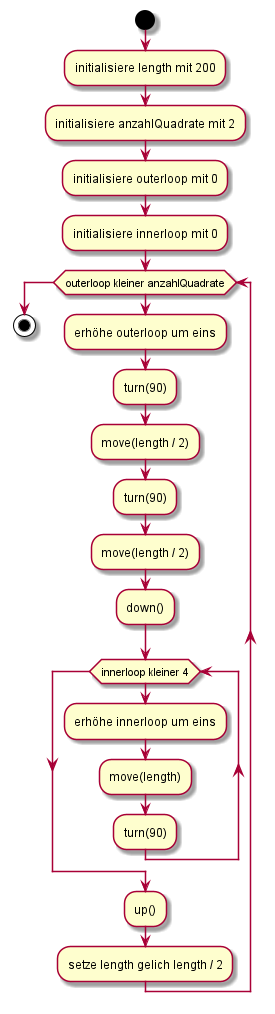
\includegraphics[scale=0.55]{uml/zweiKonzentrischeQuadrate.png}
\section{IntStack}
Schreiben Sie eine Java-Klasse IntStack, die einen ADT Stack implementiert. Die Größe (Kapazität) des Stacks soll fix sein und bei der Erzeugung eines IntStack-Objekts festgelegt werden. Intern sollen die Daten in einem int-Array abgelegt werden. Geben Sie den Source-Code ab.

\subsection{Main.java}
\lstinputlisting[language = Java , frame = trBL , escapeinside={(*@}{@*)}]{../aufgabe_08/src/aufgabe_08/Main.java}

\subsection{IntStack.java}
\lstinputlisting[language = Java , frame = trBL , escapeinside={(*@}{@*)}]{../aufgabe_08/src/aufgabe_08/IntStack.java}
\section{Aritmetischer Ausdruck}

Preoder:
	*+a/bc-d*ef\\
Inorder:
	a+b/c*d-e*f\\
Postorder:
	abc/+def*-*

\printbibliography

%%% Protokoll: Ende
\end{document}